\section*{Lecture 1: Elementary digital circuits}
The flash converter, an analog signal can be converted from analog to digital using this converter.\ it will divide a voltage into different levels, shown as the resistors on the figure below.
This will produce a truth table of sorts, if we put in a signal that is between 2 and 3 volts in the example on the blackboard, it will correspond to the 2nd row in the table below:
\begin{figure}[H]
	\centering
	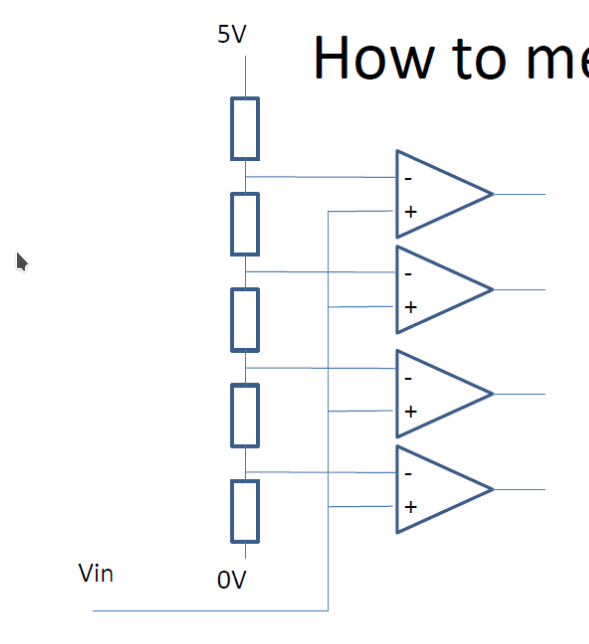
\includegraphics[width=\textwidth]{../digitalDesign/image.png}
\end{figure}
% +--------+------+
% | [0, 1) | LLLL |
% | [2, 3) | HLLL |
% | [3, 4) | HHLL |
% | [4, 5) | HHHL |
% | 5+     | HHHH |
% +--------+------+

\subsection*{Exercises}
\paragraph{1. Show by perfect induction the following relations:}

\begin{enumerate}
	\item $(A+B)*(A+C)=A+(B*C)$
	
	\begin{table}[H]
		\centering
		\begin{tabular}{|c|c|c|c|c|c|c|c|}
			\hline
			A & B & C & $A+B$ & $A+C$ & $(A+B)*(A+C)$ & $B*C$ & $A+(B*C)$ \\\hline
			0 & 0 & 0 & 0   & 0   & 0           & 0   & 0       \\\hline
			0 & 0 & 1 & 0   & 1   & 0           & 0   & 0       \\\hline
			0 & 1 & 0 & 1   & 0   & 0           & 0   & 0\\\hline
			0 & 1 & 1 & 1   & 1   & 1           & 1   & 1\\\hline
			1 & 0 & 0 & 1   & 1   & 1           & 0   & 1\\\hline
			1 & 0 & 1 & 1   & 1   & 1           & 0   & 1\\\hline
			1 & 1 & 0 & 1   & 1   & 1           & 0   & 1\\\hline
			1 & 1 & 1 & 1   & 1   & 1           & 1   & 1\\\hline
		\end{tabular}
	\end{table}
	\item $A*(A+B)=A$

	\begin{table}[H]
		\centering
		\begin{tabular}{|c|c|c|c|}
			\hline
			A & B & $A+B$ & $A*(A+B)$ \\\hline
			0 & 0 & 0   & 0       \\\hline
			0 & 1 & 1   & 0       \\\hline
			1 & 0 & 1   & 1       \\\hline
			1 & 1 & 1   & 1       \\\hline
		\end{tabular}
	\end{table}	
	\item $A+\overline{A}=1$
	
	\begin{table}[H]
		\centering
		\begin{tabular}{|c|c|c|}
			\hline
			A & $\overline{A}$ & $A+\overline{A}$ \\\hline
			0 & 1 		   & 1              \\\hline
			1 & 0 		   & 1              \\\hline
		\end{tabular}
	\end{table}	
	\item $\overline{A+B+C} = \overline{A}*\overline{B}*\overline{C}$
	
	\begin{table}[H]
		\centering
		\begin{tabular}{|c|c|c|c|c|c|c|c|c|}
			\hline
			A & B & C & $A+B+C$ & $\overline{A+B+C}$ & $\overline{A}$ & $\overline{B}$ & $\overline{C}$ & $\overline{A}*\overline{B}*\overline{C}$ \\\hline
			0 & 0 & 0 & 0     & 1                & 1            & 1            & 1   	  & 1                                      \\\hline
			0 & 0 & 1 & 1     & 0                & 1            & 1            & 0            & 0                                      \\\hline
			0 & 1 & 0 & 1     & 0                & 1            & 0            & 1            & 0                                      \\\hline
			0 & 1 & 1 & 1     & 0                & 1            & 0            & 0            & 0                                      \\\hline
			1 & 0 & 0 & 1     & 0                & 0            & 1            & 1            & 0                                      \\\hline
			1 & 0 & 1 & 1     & 0                & 0            & 1            & 0            & 0                                      \\\hline
			1 & 1 & 0 & 1     & 0                & 0            & 0            & 1            & 0                                      \\\hline
			1 & 1 & 1 & 1     & 0                & 0            & 0            & 0            & 0                                      \\\hline
		\end{tabular}
	\end{table}
\end{enumerate}

\paragraph{2. Show that the following expression is equivalent to the exclusive or function}

This is denoted by $\oplus$

\begin{table}[H]
	\centering
	\begin{tabular}{|c|c|c|c|c|c|c|c|}
		\hline
		A & B & $A * \overline{B}$ & $\overline{A} * B$ & $\overline{(A * \overline{B})}$ & $\overline{(\overline{A} * B)}$ & $\overline{(A * \overline{B})} * \overline{(\overline{A} * B)}$ & $\overline{\overline{(A * \overline{B})} * \overline{(\overline{A} * B)}}$\\\hline
		0 & 0 & 0 & 0 & 1 & 1 & 1 & 0\\\hline
		0 & 1 & 0 & 1 & 1 & 0 & 0 & 1\\\hline
		1 & 0 & 1 & 0 & 0 & 1 & 0 & 1\\\hline
		1 & 1 & 0 & 0 & 1 & 1 & 1 & 0\\\hline
	\end{tabular}
\end{table}

\paragraph{3. Reduce the following expressions:}

\begin{enumerate}
	\item $A * \overline{B} * \overline{C} + A * B * \overline{C} + \overline{A} * \overline{C}$

	$$\overline{C}(A * \overline{B} + A * B + \overline{A})$$

	\item $M * \overline{N} * P + \overline{L} * M * P + \overline{L} * M * \overline{N} + \overline{L} * M * N * \overline{P} + \overline{L} * \overline{N} * \overline{P}$

	$$M(\overline{N}*P+\overline{L}*P+\overline{L}*\overline{N}+\overline{L}*N*\overline{P})+\overline{L}*\overline{N}*\overline{P}$$

	$$M(\overline{N}*P+\overline{L}(P+\overline{N}+N*\overline{P}))+\overline{L}*\overline{N}*\overline{P}$$
\end{enumerate}

\paragraph{4. Find expressions for D and C cricuit below. What is the purpose of the circuit?}

$$C = \overline{(\overline{A(\overline{AB})})(\overline{B(\overline{AB})})}$$

$$D = \overline{\overline{A*B}}$$

This circuit is a 1-bit adder, with C being the sum, and D being the carry.

\paragraph{5. Find the Gate Input Count (GIC) of the cirquit below.}

\paragraph{6. Extend the half adder from slide 9 to take a carry as an additional input.}

\begin{figure}[H]
	\centering
	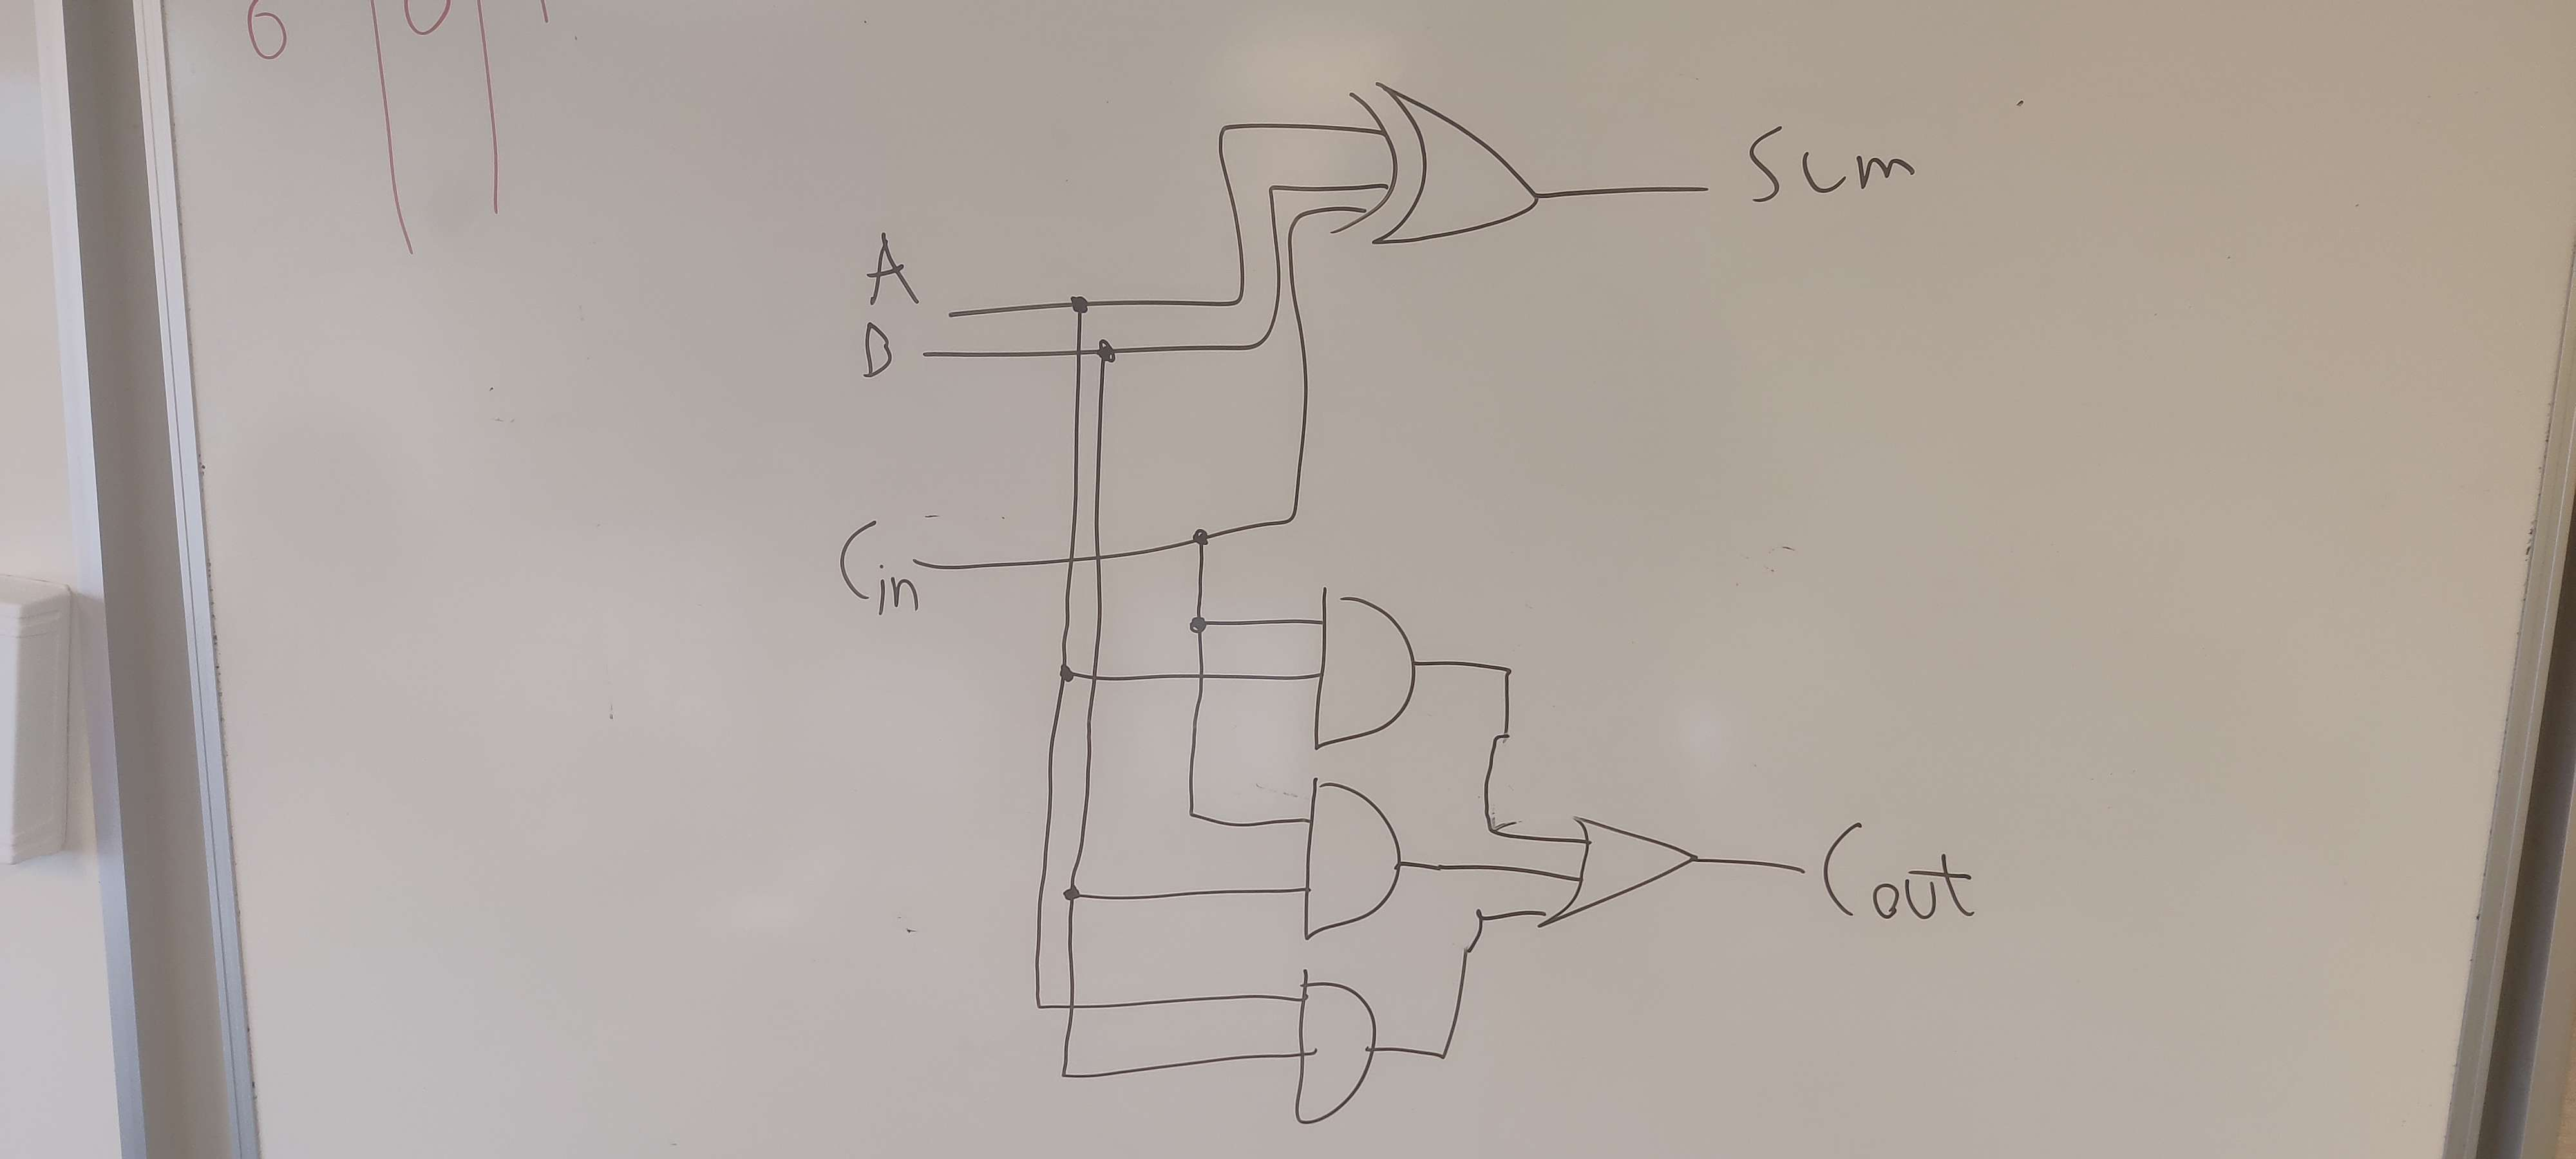
\includegraphics[width=\textwidth]{../digitalDesign/fullAdder.png}
\end{figure}